\documentclass{exam}

\usepackage{units} 
\usepackage[fleqn]{amsmath}
\usepackage{float}
\usepackage{mdwlist}
\usepackage{booktabs}
\usepackage{caption}
\usepackage{fullpage}
\usepackage{enumerate}
\usepackage{graphicx}
\usepackage{parskip}

\usepackage{2in1, lscape} 

\everymath{\displaystyle}

\author{}
\date{January 22, 2014}
\title{Statistics \\ Week One}

\begin{document}

  \maketitle
  \tableofcontents
  \section{Homework 1}

  \begin{itemize}
    \item Histograms are always counts on the y access and thing being counted on the x
      axis.   A few people did bar chart of fish oil.

    \item draw histogram of old coins

    \item bigger bin size sometimes gives more information and takes less work
  \end{itemize}

  \section{Coin Flips}

  \subsection{Normal Curve}
  Flip coin 10 times and count how many heads occur.

  \begin{figure}[H]
    \centering
    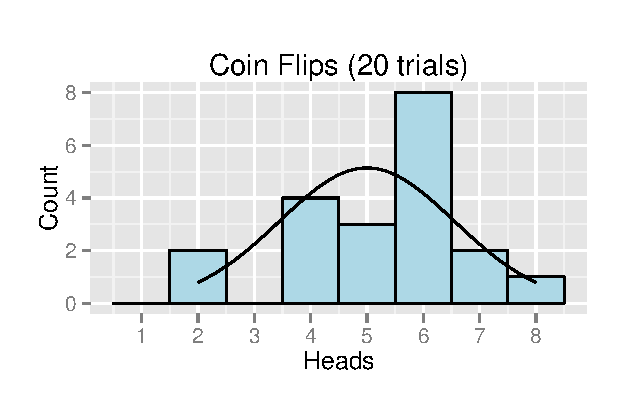
\includegraphics{figures/coins/20_10.eps}
    \caption{20 trials}
  \end{figure}

  \begin{figure}[H]
    \centering
    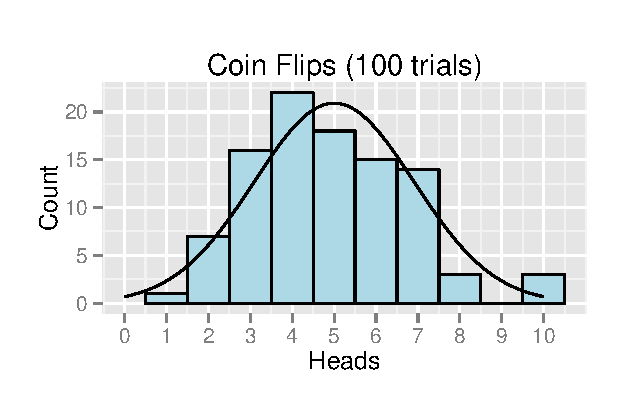
\includegraphics{figures/coins/100_10.eps}
    \caption{100 trials}
  \end{figure}

  \begin{figure}[H]
    \centering
    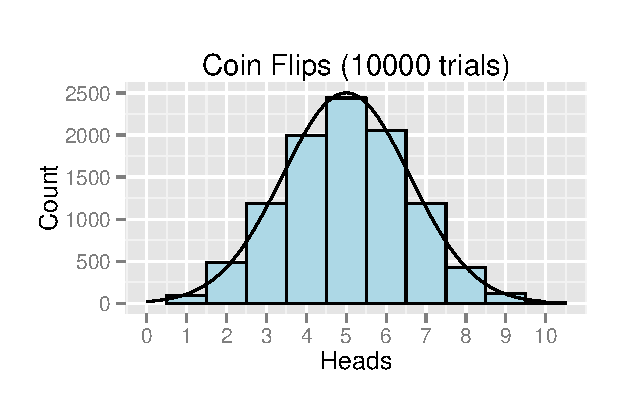
\includegraphics{figures/coins/10000_10.eps}
    \caption{10,000 trials}
  \end{figure}

  With 10,000 trials, all heads came up 8 times and all tails came up 7 times.

  \begin{table}[ht]
    \centering
    \begin{tabular}{rr}
      \toprule
      Min.    & 0.00 \\
      1st Qu. & 4.00 \\
      Median  & 5.00 \\
      Mean    & 5.01 \\
      3rd Qu. & 6.00 \\
      Max.    & 10.00 \\
      s       & 1.58441 \\
      \bottomrule
    \end{tabular}
  \end{table}

  If you divide the height of each bar by the number of trials, and add them up, the
  height of the bar is the fraction of the total with that outcome.  The sum of all the
  bar heights is 1.  Or, if each bar has a width of 1, the area of the bars is 1.

  The area is 1 because
  \begin{align*}
    A & = \sum height \\
      & = \sum \frac{count_i}{numTrials} \\
      & = \frac{\sum count_i}{numTrials} \\
      & = \frac{numTrials}{numTrials} \\
      & = 1 \\
  \end{align*}

  \begin{figure}[H]
    \centering
    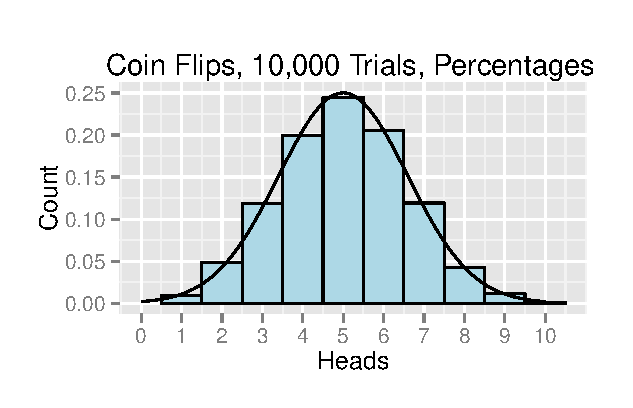
\includegraphics{figures/coins/10000_10_percent.eps}
    \caption{10,000 trials, percentages}
  \end{figure}

  If you add more flips per trial, you get more bars and the tops start to look like a
  smooth curve.  Notice that each bar is a smaller fraction of 1 since there are more
  bars.  The total height of the bars still adds up to one.

  \begin{figure}[H]
    \centering
    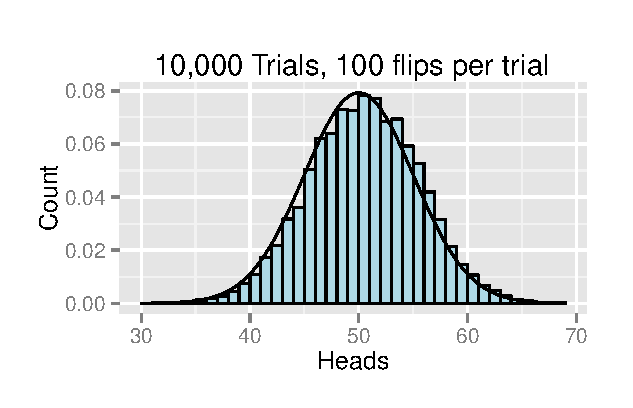
\includegraphics{figures/coins/10000_100.eps}
    \caption{10,000 trials, 100 flips per trial, percentages}
  \end{figure}

  If you replace the bars with a smooth curve, the total area under the curve is 1.

  The curve is a {\em Normal Curve}.  It happens whenever an event is either:
  \begin{itemize*}
    \item random chance (coin flip)
    \item complicated combination of factors (test, football play, height, etc.)
  \end{itemize*}

  Some characteristics of a Normal curve:
  \begin{itemize*}
    \item total area under graph is 1

    \item area between zero and some x value is probability of a value less than that
      value.

    \item symbols for mean and s when talking about Normal curves are $\mu$ and
      $\sigma$.

    \item area between $\mu - \sigma$ and $\mu + \sigma$ is about 0.68.  68\% of the
      results are in this range.

    \item area between $\mu - 2 \sigma$ and $\mu + 2 \sigma$ is about 0.95.  95\% of
      the results are in this range.

    \item area between $\mu - 3 \sigma$ and $\mu + 3 \sigma$ is about 0.997.  99.7\%
      of the results are in this range.

    \item graph changes curvature at $\mu \pm \sigma$.

  \end{itemize*}

  \subsection{Z-score}

  How to you know how likely a particular score is?  Graphs for 100 flips and 10 flips
  have different ranges on the x axis.  Heights, weights, test scores, etc., all have
  different x and y axes.

  Convert every score to a z-score.  A z-score indicates how far from the mean a score is
  in standard deviation units.

  For example, with 100 flips per trial, $s = 5.08802$.

  \begin{align*}
    z_{50} & \approx 0 \\
    z_{45} & \approx -1 \\
    z_{40} & \approx -2 \\
    z_{75} & \approx 5 \\
  \end{align*}

  A z-score of 40 is about 2 standard deviations from the mean.  About 95\% of the
  results will be between 40 and 60.

  Formula for z score is:
  \[
    z = \frac{x - \mu}{\sigma}
  \]

  Units for z-scores are standard deviations.

  \begin{align*}
    z_{50} &= 0 \\
    z_{45} &= -0.9790646 \\
    z_{40} &= -1.961765 \\
    z_{75} &= 4.917139 \\
  \end{align*}

  You can go from z-score to x by solving for x:
  \begin{align*}
    z &= \frac{x - \mu}{\sigma} \\
    x &= z \sigma + \mu \\
  \end{align*}

  What score is 2 standard deviations above the mean?
  \begin{align*}
    x & = 2 \cdot 5.08802 + 50 \\
      & = 60.12 \\
  \end{align*}

  \subsection{Finding Normal Proportions}
  Suppose you want to answer: ``What fraction of the time will I get less than 40
  heads?''

  Table of z-scores to proportions:
  \begin{table}[ht]
    \centering
    \begin{tabular}{rrr}
      \toprule
        & quantile & z-score \\
      \midrule
      1 & 0.10     & -1.28 \\
      2 & 0.20     & -0.84 \\
      3 & 0.30     & -0.52 \\
      4 & 0.40     & -0.25 \\
      5 & 0.50     & 0.00 \\
      6 & 0.60     & 0.25 \\
      7 & 0.70     & 0.52 \\
      8 & 0.80     & 0.84 \\
      9 & 0.90     & 1.28 \\
      \bottomrule
    \end{tabular}
  \end{table}

  \begin{itemize*}
    \item Table in back of book has more precision and different row/column
      arrangement to save space.
    \item table is ``what fraction is less than x'' and not ``what fraction is
      exactly x''.  With continuous things like height and weight, no fraction is
      exactly any particular value.
  \end{itemize*}

  steps:
  \begin{itemize}
    \item convert 40 to a z-score (-1.961765)
    \item look up fraction in table (0.02489493)
  \end{itemize}

  What fraction of the scores are between 55 and 65:
  \begin{itemize*}
    \item find z-scores: $z_{55} = 0.9863$ and $z_{65} = 2.9517$.
    \item find proportions in table $p_{55} = 0.8371$ and $p_{65} = 0.9984$
    \item subtract: $p = 0.9984 - 0.8371 = 0.1613$ or 16.13\%
  \end{itemize*}

  \section{Rushing Yards}

  \begin{figure}[H]
    \centering
    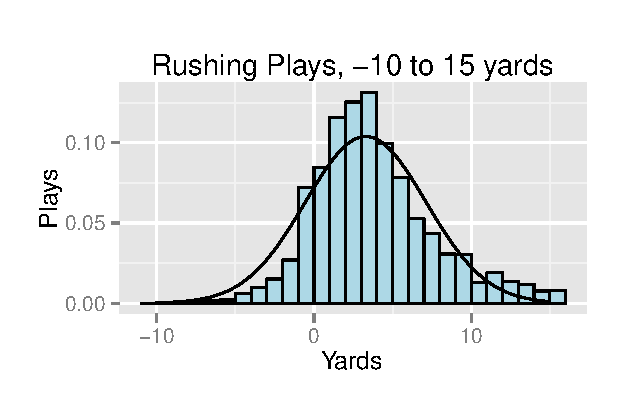
\includegraphics{figures/rushes.eps}
    \caption{Rushing yards with normal curve.}
  \end{figure}

  \begin{align*}
    \mu    & =3.287859 \\
    \sigma & = 3.839132
  \end{align*}

  If you need 5 yards for a first down, how likely are you to get it with a running
  play?

  \begin{enumerate}
    \item Compute z-score.  ($z_5 = 0.4459709$)

    \item Use table A to find proportion less than this. ($p = 0.6722$)

    \item Subtract from 1 to get proportion greater: 32.78\%

    \item Model isn't perfect.  Actual result from all plays is 30\% (fraction of
      rushing plays for more than 5 yards)

  \end{enumerate}

  What percentage of running plays lose yards?
  \begin{enumerate}
    \item Compute z-score.  ($z_0 = -0.8564068$)

    \item Use table A to find proportion less than this. ($p = 0.1959$)

    \item Actual result from all plays is 13\% 

  \end{enumerate}

  \section{Students}

  \begin{figure}[H]
    \centering
    \includegraphics{figures/students/mean70.eps}
    \caption{Hard test}
  \end{figure}

  \begin{figure}[H]
    \centering
    \includegraphics{figures/students/mean80.eps}
    \caption{Easy test}
  \end{figure}

\end{document}

